\shorthandoff{"}
\chapter{Ergebnisse und Diskussion}
\label{ch:diskussion}

\section{Analyse von Fähigkeiten und Präferenzen}
\label{ch:diskussion:analyse}
An der Umfrage unter den Projektmitarbeitern haben N=23 Angestellte des Fachbereichs \acl{JES} der EXXETA AG teilgenommen. Bei der Vorschlagsbestimmung werden folglich ausschließlich die Fähigkeiten, Präferenzen und Teamzuordnungen dieser Teilnehmer einbezogen.

Es ist festzustellen, dass die 23 Mitarbeiter insgesamt 643 Kompetenzbewertungen im Intranet des Unternehmens abgegeben haben. Das entspricht ca. 30 vergebenen Beurteilungen pro Person. Die abgegebenen Bewertungen verteilen sich auf 212 der \anzFaehigkeiten unterschiedlichen im Intranet gespeicherten Fähigkeiten. Abbildung \ref{fig:diskussion:analyse:abb1} zeigt die bewerteten Kompetenzen sortiert nach Anzahl an Beurteilungen. Dabei ist der der in Kapitel \ref{ch:empfehlungssysteme:cf:speicherbasiert} vorgestellte lange (Ratten-)Schwanz sehr gut erkennbar.

\begin{figure}[h]
	\centering
	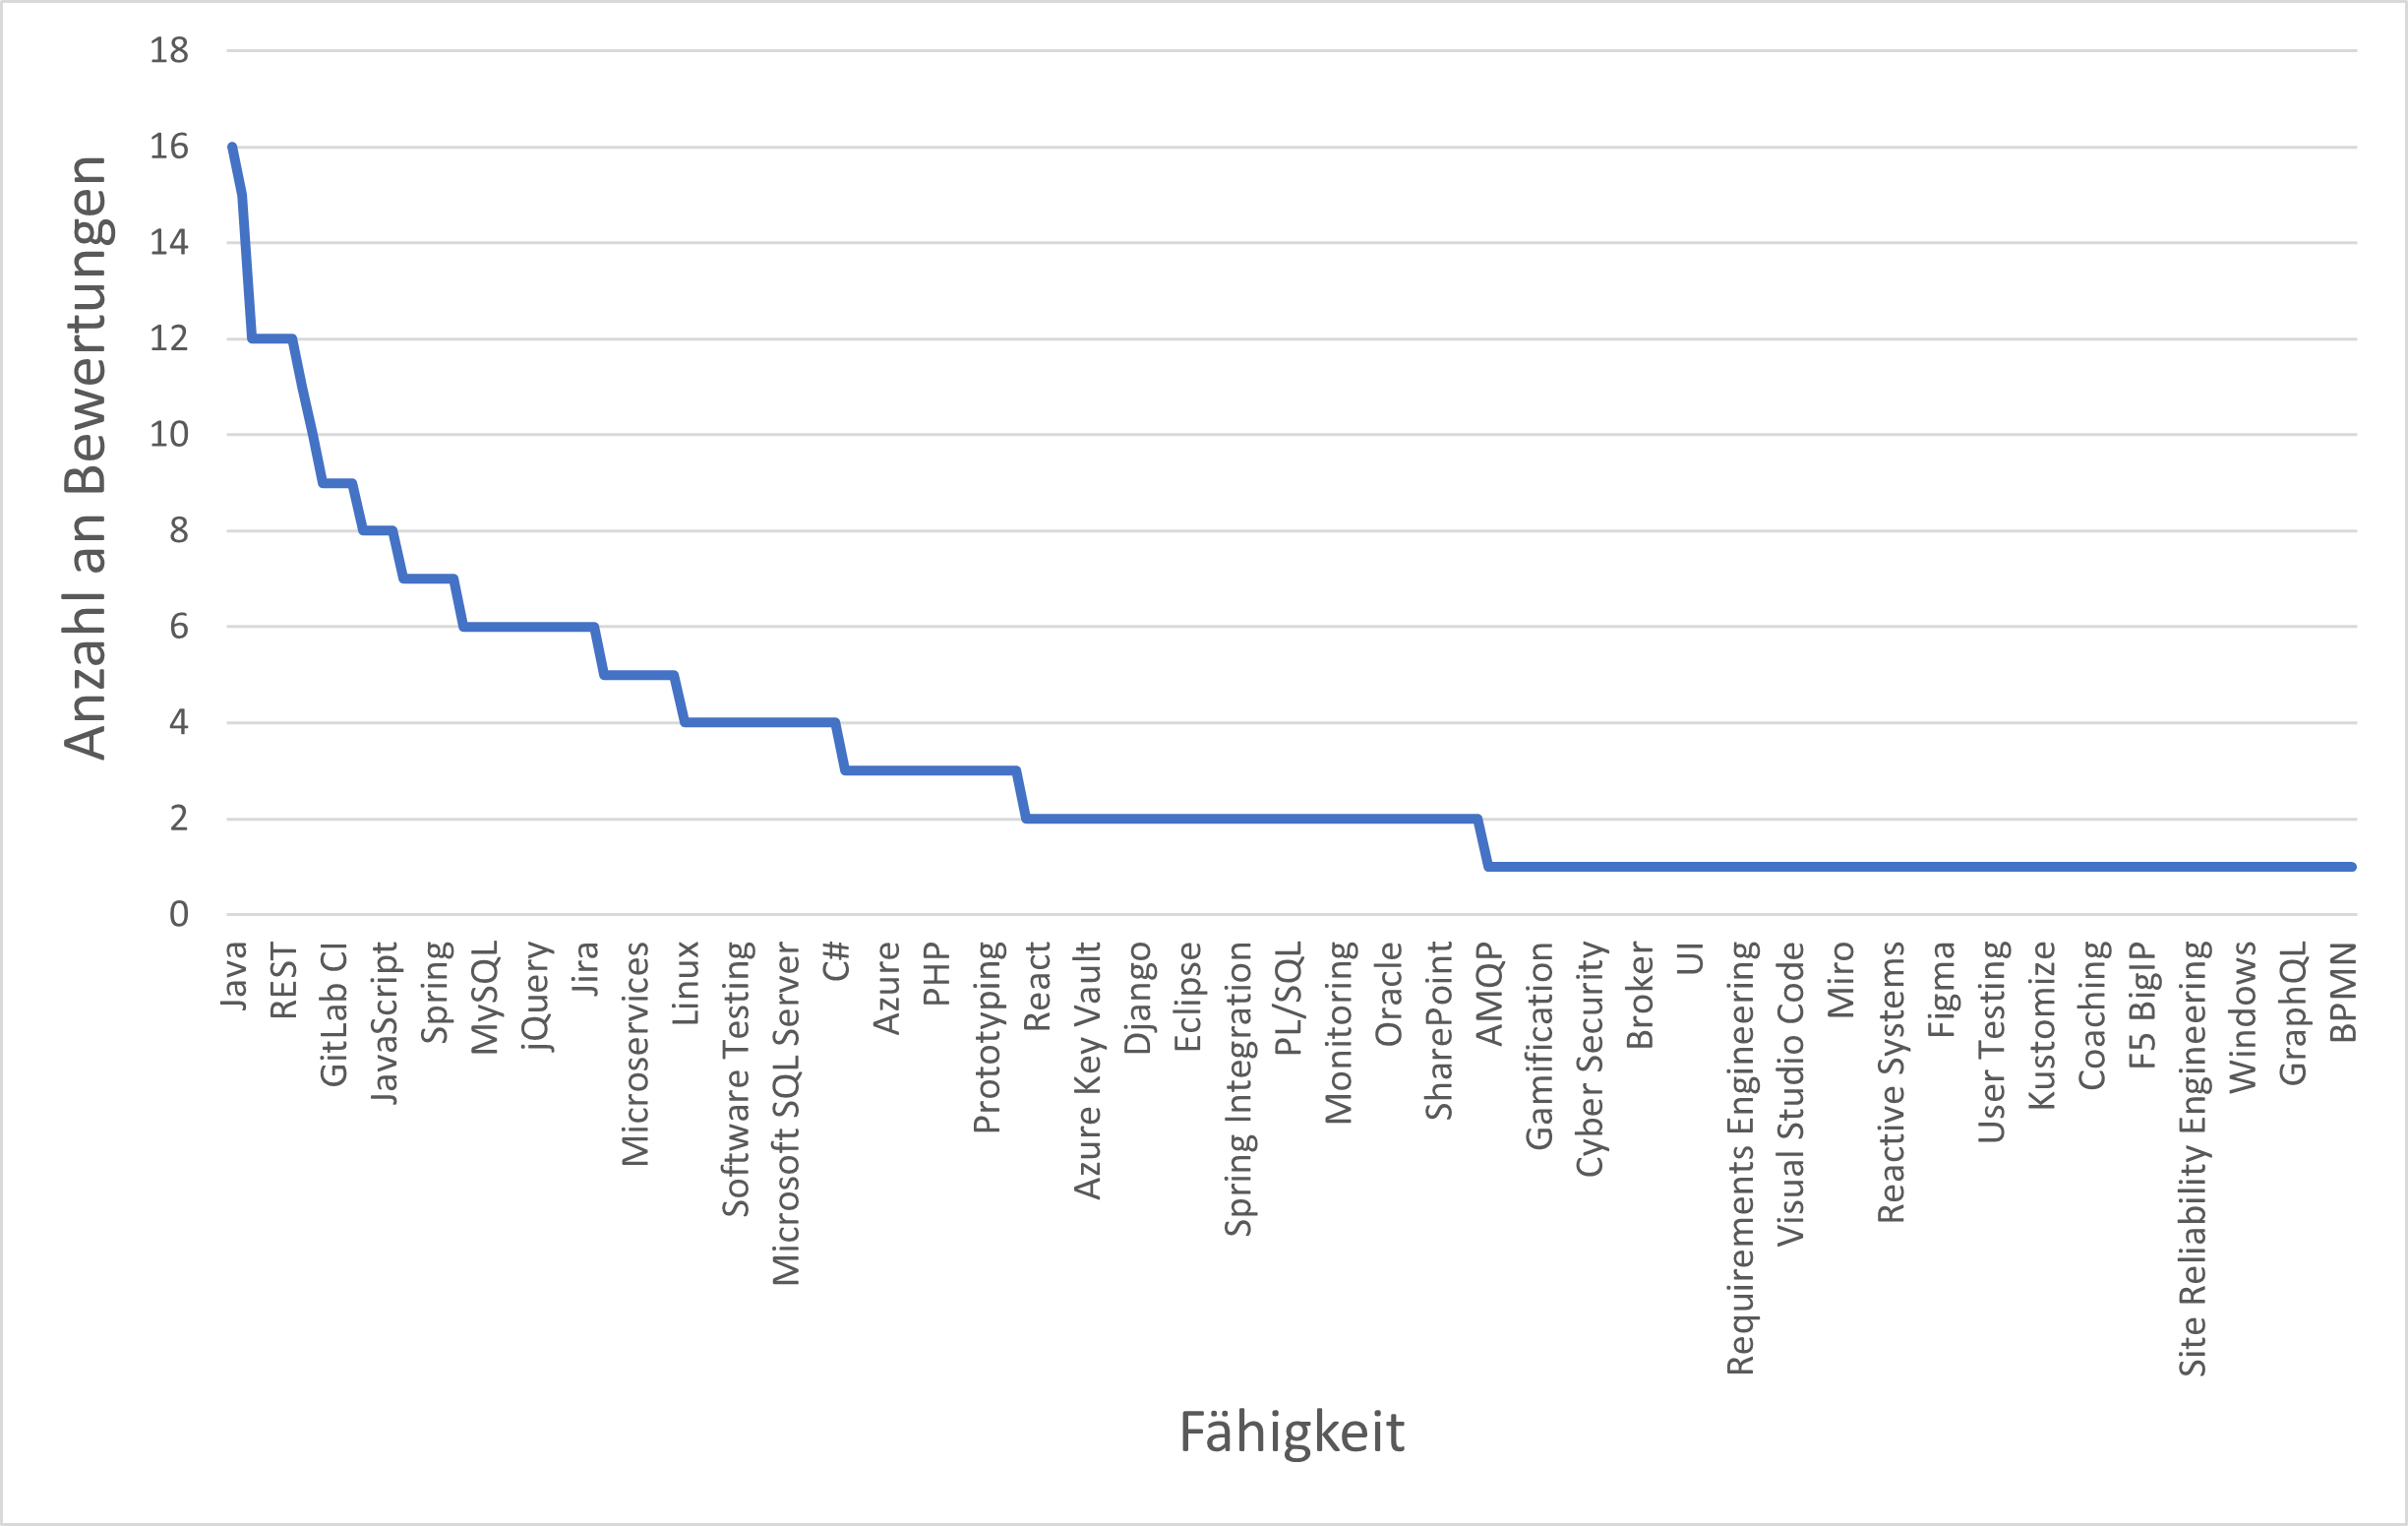
\includegraphics[width=1\textwidth]{gfx/long-tail-intranet.png}
	\caption{Langer (Ratten-)Schwanz bei den Fähigkeitsbewertungen im EXXETA-Intranet}
	\label{fig:diskussion:analyse:abb1}
\end{figure}

In Abbildung \ref{fig:diskussion:analyse:abb1} ist zu erkennen, dass Java mit 16 Beurteilungen die meist bewertete Fähigkeit im Fachbereich ist. Bezüglich des langen (Ratten-)Schwanzes
\newpage

Long Tail: 9 Fähigkeiten haben 10 oder mehr Bewertungen --> Entspricht ca. 4,25 Prozent; 151 Fähigkeiten haben 3 oder weniger Bewertungen --> Entspricht ca. 71,23 Prozent. Meisten Bewertungen erhielt Java mit 16 Bewertungen, dicht gefolgt von Spring Boot mit 15 Bewertungen. Long Tail auch bei grafischer Darstellung der Fähigkeiten zu erkennen:



Kaltstart: 4 Nutzer (17,39 Prozent) haben gar keine Fähigkeiten angegeben / Es sind immer mind. 19 andere Personen auf einem Skill verbunden

\newpage
Projekt A: unilateral/bilateral\\
Projekt B: bilateral/unilateral\\
Projekt C: bilateral/unilateral\\
Projekt D: unilateral/bilateral\\
Projekt E: unilateral/bilateral

- Link aufs Intranetprofil

\shorthandon{"}
